\section{Overall Description}

\subsection{Product perspective}
 %Describes the environment of the system

\subsubsection{Description}
SMSEncryption is a new product which can be used in conjunction with any mobile text manipulation application, such as the general keyboard input used by the different mobile operating systems, or any other text manipulating application, capable of using the basic GSM character set - should you require encryption and decryption functionality for secure communication between two parties.
\vspace{12pt}\\
The GSM character set contains a limited amount of characters, which will, in turn, limit the encryption methods we can make use of, as many encryption algorithms greatly increase both the size of the message, and the number of different characters used. Making use of these encryption algorithms that generate large amounts of characters will be infeasible, as sending large SMSes will be expensive.
\subsubsection{System interfaces}

\subsubsection{User interfaces}
 The user interface is what will allow the user to type a message, encrypt it, copy the ciphertext, and paste it into the application that will send the message. On the receiving end, the message received will be copied, and pasted into the SMSEncryption application, which will be used to decrypt the received message. This ensures integrity of the message, as only users of the application will be able to encrypt/decrypt the message in the agreed upon way.
\subsubsection{Hardware interfaces}
The software will run on a mobile device that allows user interaction and text manipulation.
\subsubsection{Software interface}
 The software interface will make use of operating system features, such as a clipboard on the device to facilitate 'copying' and 'pasting' of texts or ciphertexts.
\subsubsection{Memory}
The device needs minimal storage space on the device for a local database and the application is 2mb large.
\subsubsection{Operations}
\begin{itemize}
\item User-initiated operations:
\begin{itemize}
\item Create user account
\item Edit user account
\item Add contact
\item Edit contact
\item Remove contact
\item Enter message
\item Encrypt message
\item Decrypt message
\item Synchronise contact
\end{itemize}
\end{itemize}


%Note:
%Required : Functionality must be provided if service is provided
%Extends : Extended functionality which can be provided, but not always.
\subsubsection{Use Cases}
SMSEncryption Use case diagram

\begin{center}
 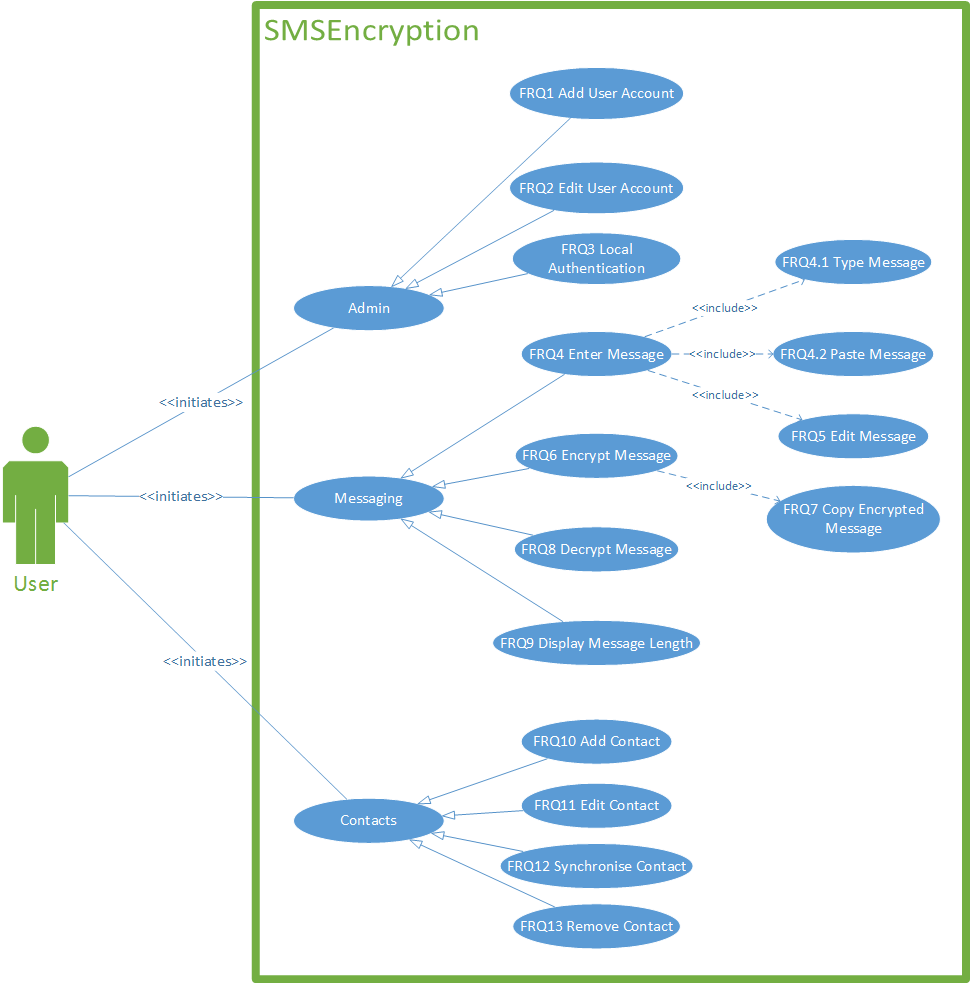
\includegraphics[width=13cm]{diagrams/UseCaseDiagrams/UsecaseV5.png}
\end{center}

\subsubsection{State Diagram}
SMSEncryption State diagram

\begin{center}
 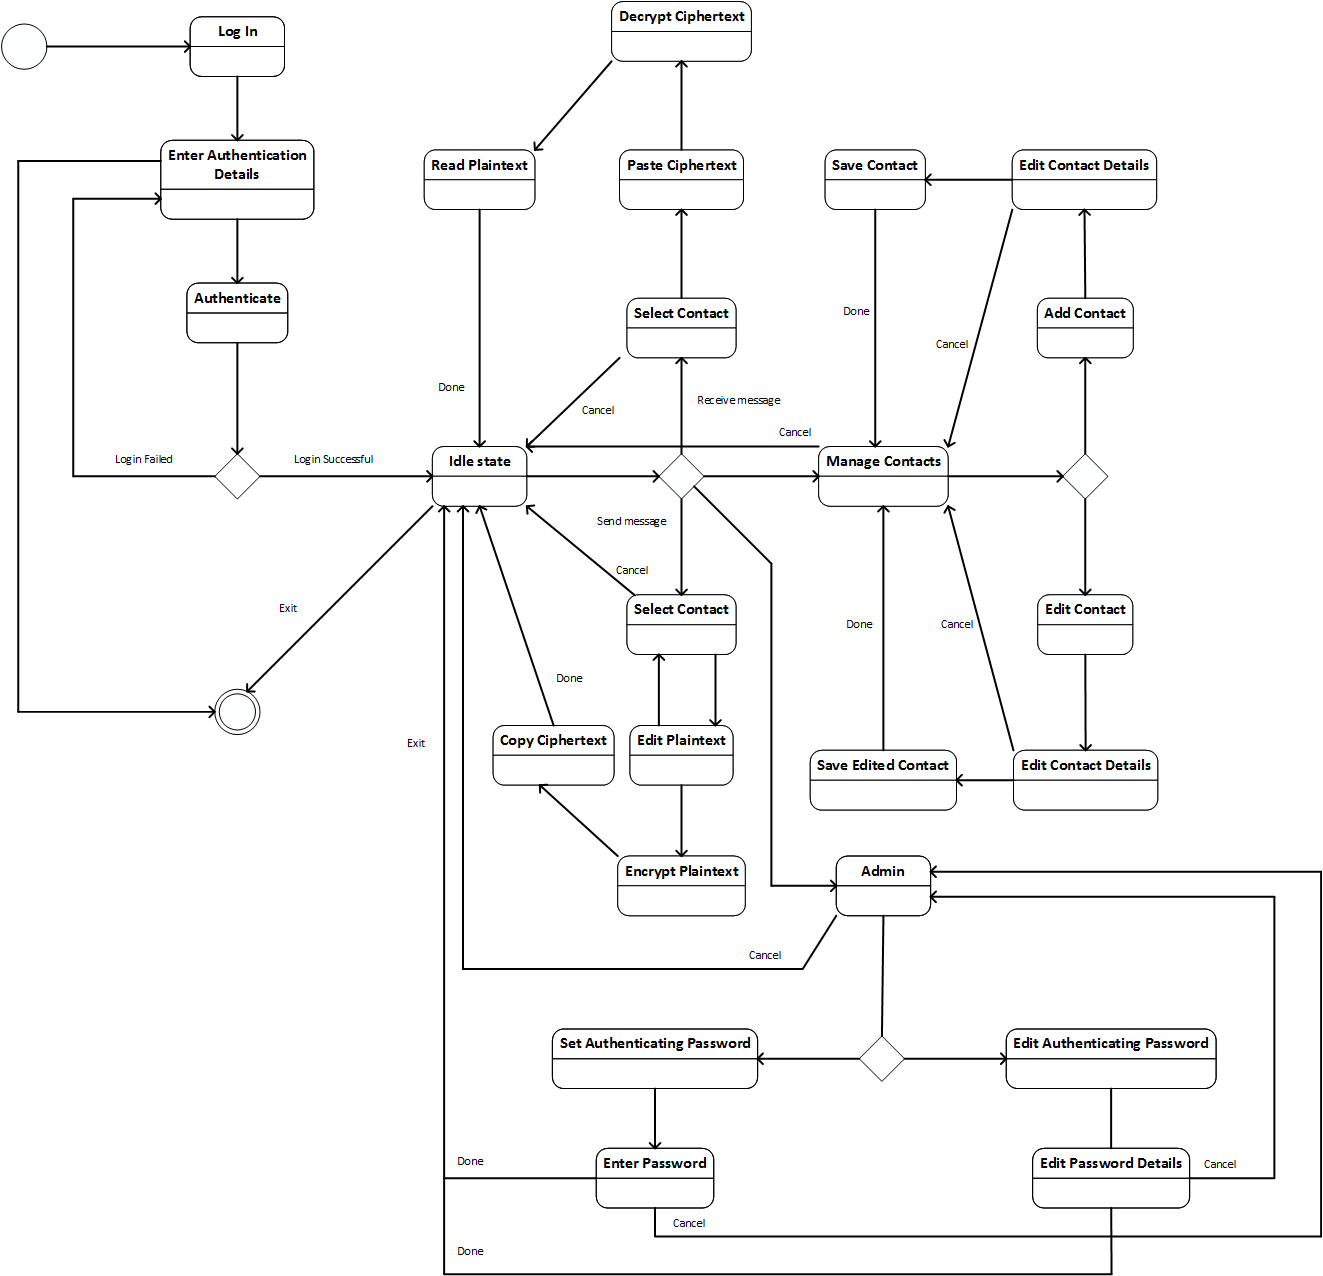
\includegraphics[width=13cm]{diagrams/StateDiagrams/SMSEncryptionStateMachine.png}
\end{center}


\subsection{Product functions}
The application is devided int 3 core functionalities, Admin, Messaging and Contacts.

\subsubsection{Admin}
\begin{itemize}
\item The user shall be able to make an account.
\begin{itemize}
\item On first use of the application, a username password must be created that will ensure user authentication.
\item Only one account is allowed per device.
\end{itemize}
\item The user shall be able to edit his/her account.
\begin{itemize}
\item Should it be required, once logged in the user can edit his/her account details.
\end{itemize}
\item The application shall make use of local authentication to log in.
\begin{itemize}
\item Every time a user wants to use the application, the password must be provided along with the login details.
\item If the provided password (and related details) are entered correctly, the user may gain access to the application.
\item If the password provided remains incorrect after three times, the application will lock for a specified time - preventing access from an unauthorised user.
\end{itemize}
\end{itemize}

\subsubsection{Messaging}
\begin{itemize}
\item A message shall be able to be entered via either typing or pasting it in.
\item A message shall be able to be edited once it has been entered.
\item A message shall be encrypted.
\begin{itemize}
\item The user will select a relevant contact, that contacts details will then be used to perform encryption.
\end{itemize}
\item A message shall be copyable once it has been encrypted.
\begin{itemize}
\item The encrypted message (ciphertext), can then, by the user, be copied out and pasted into the application that will send the ciphertext to the desired receiver; via any messaging method.
\end{itemize}
\item An encrpyted message received and entered into the application shall be decrypted.
\begin{itemize}
\item The desired receiver will be able to decrypt the message back into its plaintext.
\end{itemize}
\item The message length shall be displayed.
\begin{itemize}
\item This is to ensure message length does not exceed 144 characters.
\end{itemize}
\end{itemize}

\subsubsection{Contacts}
\begin{itemize}
\item A contact shall be added.
\begin{itemize}
\item In order for communication to take place between two devices they need to be synchronized.
\item A user adds what is called a contact, it will ask the name of the contact as well as generate a unique word to be provided to the other person and an input box where the unique word appearing on the contacts phone must be input.
\item Both users must add each other at the same time, because they need each other's unique word that will be generated for their communication. This will synchronize communication between the devices.
\end{itemize}
\item A contact shall be editable once added.
\item A contact shall be removable once added.
\item A contact shall be resynchable once added.
\begin{itemize}
\item Once a contact has been added, you can resynchronise with that contact at any time in the future should you require this.
\end{itemize}
\end{itemize}

\subsection{User characteristics}
%Assumptions about the users, their background, how
%much training they will need
%? e.g., different user interfaces for expert vs. novice users
%? Only user characteristics that affect the software
%requirements
\begin{itemize}
\item There will be only one user class who will have full access to all the features provided by the application after local authentication.
\item It is assumed that the user has proficient knowledge on how to copy items from messages such as SMS and paste it within this application.
\item It is also assumed that the users performed the device synchronization phase correctly as there is no way for the device to know.
\end{itemize}


\subsection{Constraints}
%Anything that will limit the designer's options
\begin{itemize}
\item The encrypted message length will be limited to 160 characters.
\item The application must make use of the basic GSM character set.
\end{itemize}



\subsection{Assumptions and dependencies}
%List any assumed factors (as opposed to known facts) 
%that could affect the requirements stated in the SRS. 

\begin{itemize}
\item It is assumed that the amount of characters in the basic GSM character set is 128 for the 7-bit encoding used in GSM.
\item It is assumed that the devices being used allows for copy and pasting of text between different interfaces and applicaitons.
\end{itemize}


\subsection{Apportioning of requirements}
The following are possibilities that can be added to future versions of the sytem:
\begin{itemize}
\item SMS capability from within the application.
\item Compatibility for other operating systems.
\end{itemize}